
% SEP 2012 Group 13
% Software Requirements Document (SRS)
%
\documentclass[11pt, a4paper]{report}
\usepackage{graphicx}
\usepackage{fullpage}
\usepackage{url}
\pagestyle{headings}

%%% page parameters
\headsep = 25pt
\begin{document}
\oddsidemargin -0.5 cm
\evensidemargin -0.5 cm
\textwidth 15 cm
\topmargin -1.2 cm
\textheight 25 cm
\begin{center}

\includegraphics[scale=1.5]{./UniLogo}\\[1cm]    
\textbf{\Huge \bfseries User Manual}\\[1.5cm]
\textbf{\huge for}\\[0.5cm]


% Title
\textbf{ \huge Archaeology Robot }\\[0.3cm]
\textbf{ \huge Team 13 }\\[2cm]


\begin{tabular}{ |c | p{2cm} |}
	\hline
Yufeng Bai 1600095 & \\[.5cm] \hline
Jun Chen 1206265 & \\[.5cm] \hline
Dawei Geng 1219181 & \\[.5cm] \hline
Yunyao Yao 1203525 & \\[.5cm] \hline
Shikai Li 1214223 & \\[.5cm] \hline
Quang Khoi Nguyen 1187070  & \\[.5cm] \hline
Yatong Zhou 1204471 & \\[.5cm] \hline
\end{tabular}


\vfill

% Bottom of the page
Version 1.0 \\ [0.2cm]
{\large \today}

\end{center}


\tableofcontents



% Version History %

% IMPORTANT %
% Whenever you make a change to this document you MUST put an entry in below
% Must conform to firstName lastName &  date & discription \\ \hline


\clearpage
\section*{Revision History}
\begin{tabular}{| l | l | l | l | }
\hline
Name      		&	Date        	&	Reason For Changes                  	&	Version     	\\ \hline
Dawei Geng      & 	12 Aug 2012    	& 	basic framework of the SRS     			&	0.1             \\ \hline
Dawei Geng      &	12 Aug 2012    	& 	Introduction and Overall Description    &	0.1             \\ \hline
Yufeng Bai  	&	13 Aug 2012 	&	User requirements 						&	0.2  			\\ \hline
Dawei Geng		&	16 Aug 2012		&	Add user requirements \& layout edit	&	0.3 			\\ \hline
Dawei Geng		&	17 Aug 2012		&	Minor changes \& layout edit			&	0.3.1 			\\ \hline
Yatong Zhou\&Shikai Li		&	17 Aug 2012		&		External Interface Requirements		&	0.4			\\ \hline
Jun Chen\&Yaoyun Yao		&	18 Aug 2012		&		Other Non-Functional Requirements	b&	0.5			\\ \hline
Nguyen Quang Khoi			&	18 Aug 2012		&		System Features			&	0.6				\\ \hline
Jun Chen	&	2 Oct 2012		&	fixing chapter 1 accroding to the feedbacks			&	0.8			\\ \hline
Jun Chen	&	2 Oct 2012		&	fixing chapter 2 accroding to the feedbacks			&	0.8 			\\ \hline
Jun Chen	&	6 Oct 2012		&	fixing chapter 3 accroding to the feedbacks			&	0.8 			\\ \hline






\end{tabular}
\clearpage

% Introduction %

\chapter{Introduction}

\section{Purpose}
This document is set to describe the requirement of the Archeology Robot Project, to be used for survey an archaeological site containing the remnants of an ancient city. This document shall address the user requirements, system features, external interface requirements and other non-functional requirements describing the robot and the control software's function. 


\section{Document Conventions}
In this document, user requirements will be describe with requirement description, requirement rationale, acceptance criteria, source of the requirement and a priority ranking. However, other requirements such as external interface requirements and non-functional requirements may not have priority ranking. 

The requirements will be labeled with ID which contains letter representing the type of the requirement and a reference number. U, S, UC and N will be used in this document corresponded to User Requirement, System Requirement, Use Case, and Non-Functional Requirement.  The reference number which is following the letter is sequential.



\section{Intended Audience and Reading Suggestions}
The audience of this document can be project managers, developers and testers of this project. 
\begin{itemize}
\item For project managers, this document gives a overall description to the requirements. A project manager shall read the entire document and pay special attention to User Requirements, External Interface Requirements, and Non-Functional Requirements.
\item For developers, this document gives details about the requirement for them to work on. A developer shall reader the entire document and pay special attention to Use Cases and Non-Functional Requirements. 
\item For testers, every requirement has a acceptance criteria which can be used to help all the test, and testers also should focus on the User Requirements. 
\item For clients, this document gives them details about the requirements they want. Clients can read this document to know the project is satisfied or not. They can also add anything that this document does not mention. 
\end{itemize}


\section{Project Scope}
This project's aim is to develop a new intelligent Archeology Robot to be used for survey an archaeological site. A graphic user interface shall be developed for navigation and keep track of the burried remnants within the site. The user interface will also shows the details of the robot and its position and conditions. The robot will be connected to a host computer over Bluetooth connection. The robot shall be allowed to automatic scan all the flat surface on the site and be able to find the hidden walls or remnants under the ground and produce the information of the site and shows on the user interface's map. 
User can operate robot through operating the host machine. Manual control shall be enabled when required.


\section{References}
\subsubsection*{Design Brief}
Computer Science Department, The University of Adelaide (2012) \textit{Project Description}. Adelaide : South Australia

\subsubsection*{Minutes of internal meeting}
The minutes of internal meeting of team 13.

\subsubsection*{Minutes of client meeting}
The minutes of client meeting of team 13.

\pagebreak


% Overall Description %

\chapter{Overall Description}

\section{Product Perspective}
The goal of this project is to develop a new archeology robot and its operating software. It will contains the robot itself, a host machine with a GUI connect to the robot over Bluetooth. This robot will be able to survey the archaeological site with safety priority which the robot shall have the ability to avoid walls and obstacles on the surface. 

The robot itself will have one light sensor to detect the hidden walls and object, two touch sensor to avoid collision, and ultrasonic sensors to detect walls or obstacles in front of the robot. 

The operating software will have a user friendly GUI which contains control panel, map area, and robot detail information such as battery usage, location, and mode. 

The database of this project shall contain XML map files of the sites which the robot have surveyed before. Saving and loading of these files is allowed. 

\section{Product Features}
The project includes the following main features
\begin{itemize}
\item Robot shall automatic scan the site and giving feedback on to the screen of the host machine in real time. 
\item A site map shall be produced when a complete survey is done by the robot.
\item Users can save and load maps via the operating software of the robot. 
\item Manual control over the robot is allowed. 
\item Since there may have “no go” zone within the site. The robot shall never enter the “no go” zone, if ever a robot is in a “no go” zone by accident, a message will displayed on the host's screen and called for help.
\item Users have the ability to add and remove "no go" zones via the operating software of the robot.
\item As the robot is working on the site, safety is important. In order to ensure that, the robot should avoid any bumps.
\end{itemize}

\section{User Classes and Characteristics}
The user of this system will be trained archaeologist who have the knowledge to operate and control the robot. These archaeologist have been trained to perform safe operations to the software and the robot under variety of situations.

\section{Operating Environment}
The host software can be run on any system which has installed, Java JRE, NXJ and also have Bluetooth implementations.
The client software shall be installed on a LEGO\textregistered{} Mindstorm\textregistered{} robot running NXJ 0.9.1.

\section{Design and Implementation Constraints}
The client machine which is the robot shall have its own program can accept and run commands from the host machine. The client software shall be stored in the robot's memory which has limited capacity. Therefore the software on the client end needs to be as minimal as possible.
The software shall be written in JAVA using the LeJOS API to interact with the robot.
The client and host shall use Bluetooth\textregistered{}  for communications.

\section{User Documentation}
A user manual shall be produced, outlining the basic operation of the robot and also going into detail about the full capabilities of the operating software.


\section{Assumptions and Dependencies}
In the project the following list will be assumed.

\begin{itemize}
  \item{The terminal used is capable of running Java SE 6}
  \item{The terminal used is capable of running leJOS NXJ 0.9.1}
  \item{The terminal used is capable of Bluetooth connection}
  \item{The archaeological sites will be a single enclosed polygon}
  \item{The archaeological sites will have grind lines ever 50mm both vertically and horizontally}
  \item{The archaeological sites will be a flat ground}
  \item{Hidden walls will be showed as gray shape}
  \item{Obstacles will be showed as brown shape}
%  \item{No-go zone will be showed as red shape}%
  \item{The smallest hidden walls which a robot can detect will be at size of 25mm*25mm}
  \item{The smallest External objects which a robot can detect will be at size of 75mm*75mm}
\end{itemize}


\pagebreak



% User Requirements %

\chapter{User Requirements}
%User requirements should consist of functional requirements which the system should provide.
\section{Manual Controls}
\subsection{R0001: Robot movements}
\paragraph{Description: }
Robot shall be able to move forward, backward, rotate left and rotate right according to the manual operation.
\paragraph{Rationale: }
 If user choose the manual mode, the robot will not be permitted  to move by itself. The user is required to use the GUI to control the robot by pressing the button. The GUI has different buttons which represent the different functionality. As the manual controls are the first stage of the robot development, it will impact the auto mode of the robot. This requirement is used to ensure the movements of the robot are working properly. With the implement of manual control, users (clients) can control the robot in the way the want. In emergency, the user can stop the robot via pressing buttons on the GUI, this requirement will also improve the safety coefficient. 
\paragraph{Acceptance criteria: }
In manual control mode, when user press direction button(forward, backward, left, right) on the GUI, the robot will move according to the command which is given by GUI. The robot is able to move correctly.   
\paragraph{Source: }
 Introduction of Project Description
\paragraph{Priority: }
High



\subsection{R0002: Hidden wall (below ground) detection}
\paragraph{Description: }
The robot is required to search the map and to find all hidden walls (below ground). In manual control mode, the user need to control the robot to detect by itself.
\paragraph{Rationale: }
The robot will not be allowed to detect the hidden walls automatically. User have to use GUI to control the robot. If the users do not give the command  to the robot. The robot will stop and wait for the further command. The switch of light sensor is still controlling by users. If users do not turn the light sensor on, the robot will not be able to find the hidden walls.  
\paragraph{Acceptance criteria: }
When the users control the robot by GUI, the light sensor will be on once the robot is on. The light sensor will detect the hidden walls according to the colours of the shape on the map. If the shape is black, this shape will be detected as a hidden wall. When robot traverse the map(light sensor is on), if the robot find a hidden wall(black shape), it will remind the users and let the users give it the further command.
\paragraph{Source: }
 Introduction of Project Description
\paragraph{Priority: }
High



\subsection{R0003: Avoid entering the no-go zone}
\paragraph{Description:}
The robot must be sure to work safely. So the robot is not allowed to enter the no-go zone.
\paragraph{Rationale:}
 The robot must walk inside the map and not go into the no-go zone.  No-go zone is the zone with potential danger to the robot, so the robot must not enter no-go zone for safety reason.
\paragraph{Acceptance criteria:}
 In this situation, if the robot detect the no-go zone, the robot will remind the user, at the same time it will slow down automatically and stop in front of the no-go zone. Then the robot will not allow to move forward until the users give it move command.
\paragraph{Source:}
Project Description 2.4 safety.   
\paragraph{Priority:}
High


\section{Automatic Survey}
\subsection{R0003: Automatic robot movements }
\paragraph{Description:}
The robot is able to move forward, backward, rotate left and rotate right automatically. The users do not need to control robot and robot can traverse the whole map safely and effectively.
\paragraph{Rationale:}
The movement is the fundamental requirement for the robot. Robot must move and traverse the whole map by itself. In this mode, user do need to use the GUI to control the robot, the robot will move automatically.    
\paragraph{Acceptance criteria:}
The robot can move automatically. It can determine to move forward or rotate according to the actual situation of map by itself. The automatic mode also can be switched by users' operation.  
\paragraph{Source:}
 week 3 of the milestone plan. 
\paragraph{Priority:}
High



\subsection{R0004: Automatic exploration}
\paragraph{Description:}
The robot is required to search the map and to find all hidden walls (below ground). In automatic mode, the robot is required to traverse and find hidden walls automatically. When the robot discover one hidden wall, it will record the position of the hidden wall and choose another direction.
\paragraph{Rationale:}
The main task of this robot is to find the hidden wall on an archaeological site. The robot must have the ability to detect all areas and find all hidden walls without the controlling.   
\paragraph{Acceptance criteria:}
The robot need to traverse the site(except the no-go zone). The light sensor will take responsibility to detect the hidden wall. The light sensor will find hidden walls according the colour of the them(black shape). Users do not need to control the sensor. The sensor will keep switching on for the whole process. When the robot find one hidden wall, it will record the position of this wall and send the message to users, at the same time , the robot will choose another direction and keep detecting.  
\paragraph{Source:}
 Introduction of Project Description
\paragraph{Priority:}
High



\subsection{R0005: Avoid collision}
\paragraph{Description:}
The robot must be sure to work safely. The robot is not permitted to collide against any external objects.
\paragraph{Rationale:}
The robot is not permitted to bump to any external object. So the robot will use light sensor and bump sensor to avoid colliding with any external objects.
\paragraph{Acceptance criteria:}
When the robot is on, the light sensor and bump sensor will be on as well.The bump sensor and ultrasonic sensor will keep switching on for the whole process. In this situation, if the robot detect the external block, the robot will remind the user, at the same time it will slow down automatically and stop in front of the block(the colliding is forbidden, so we have to set it stop automatically) Then the robot will choose another direction and travel another way.
\paragraph{Source:}
Project Description 2.4 safety.  
\paragraph{Priority:}
High


\subsection{R0006: Finding path }
\paragraph{Description:}
The client hopes the robot is able to find the path between two given position. In the automatic mode, the robot need to calculate the path(the shortest and safest path are better).    
\paragraph{Rationale:}
This is the additional requirement from client, the client hopes we can implement this task. According to the client's requirement, we should find the shortest way or the safest way(safe is priority) to reach to a given position. 
\paragraph{Acceptance criteria:}
The user can set the position by GUI, then the robot will calculate the path automatically and move on the map according to client's requirement. In our design, safe is priority, so the robot will be chosen to go the way without no-go zone, also the robot will not go to outside of the map. Moreover, the way be chosen should have less obstacles so that the robot will have less chance to be damaged.(when client system error occurs)  So we always choose the safe way first.    
\paragraph{Source:}
 Minutes of the first client meeting   
\paragraph{Priority:}
Low


\section{Graphical User Interface}
\subsection{R0007: Map representation}
\paragraph{Description:}
The GUI contains a window for drawing the map. The map is synchronous with the robot. Before the  robot starts, the initial colour of map window is black. When the robot moves, the map will be drawing gradually. After the robot finishes the detection, the map will be finished at the same time. The the GUI will remind users that the map is complete. The GUI will use some colors to represent the component of the map: black for the unexplored Area, red for the no-go zone, yellow for the Buffer zone, gray for the hidden wall(underground wall) and brown for the Obstacle (above-ground wall).
\paragraph{Rationale:}
The map window is used for users to show the process of detection. From the map window, the users can check the position of each hidden wall, Obstacle and the “no go” zone. Also they can check the zones that are explored or not. Map is necessary and convenient way to view the survey result because it is easier for user to read it. With the map representation, the survey result will be shown effectively.
\paragraph{Acceptance criteria:}
When the robot moves, the map will be drawn gradually. The map will mark all hidden walls, blocks and "no-go zones". The map also demonstrates the location of the robot, which is convenient for users to understand whole process of searching.
\paragraph{Source:}
Project Description 2.1
\paragraph{Priority:}
High



\subsection{R0008: Robot representation}
\paragraph{Description:}
The status of robot need to be represented to users. The status includes the power of battery(%), the location(x,y), the Bluetooth connection(activated, inactivated) and the speed of the robot(0-10). Users are able to understand the  robot's situation and make some adjustment.
\paragraph{Rationale:}
When the power of battery is almost running out (below 20%), the robot need to return to where it begins. So it is necessary to monitor the status of battery. The location and the speed demonstrate the immediate situations for robot. The Bluetooth connection is the signal to represent the signal of Bluetooth to make sure the robot is connecting correctly.
\paragraph{Acceptance criteria:}
The battery is demonstrated by GUI using a bar. We will use percentage to show how much power left. The location is demonstrated by coordinate to show where the robot is. 
The speed is demonstrated by GUI using a bar and a number. 
The Bluetooth connection is a light, when the Bluetooth works properly, the colour of  light will be green. If the Bluetooth lose the signal, the colour will become red.
\paragraph{Source:}
 Project Description 2.1
\paragraph{Priority:}
Low



\subsection{R0009: Robot mode change}
\paragraph{Description:}
There are two modes can be switched by users: Manual mode and Automatic mode. These two modes can be switched between each other in GUI. 
\paragraph{Rationale:}
The client requires us to have these two modes, which is convenient for the client to control the robot at any time. If we do not have the functionality of mode change, the client will hard to control the robot. The mode change will be built as two buttons. One is for the manual mode and the other is for automatic mode.
\begin{figure}[ht]
\centering
\setlength\fboxsep{2pt}
\setlength\fboxrule{0.2pt}
\fbox{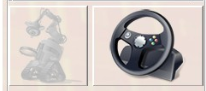
\includegraphics[width =0.8\linewidth]{robot_mode_change}}
\caption{Buttons for mode change}
\label{sec:NXJCC}
\label{fig:NXJCC}
\end{figure}

\paragraph{Acceptance criteria:}
When the users press the button of mode change, there is a window jumping out and write like “Do you want to change to the manual mode?” If the users press “yes”, the robot will execute as manual mode. The same situation is also suitable for manual mode to automatic mode.
\paragraph{Source:}
 Minutes of the first client meeting 
\paragraph{Priority:}
High 


\subsection{R0010: User mode change}
\paragraph{Description:}
There are two modes can be switched: Client mode and Maintenance mode. In Client mode, this system allow client to control the robot by GUI, the client can use the robot to search the archeological site and to find the hidden walls, blocks and the no-go zones. The client is not permitted to edit the setting of the robot, for example, the client is not allowed to change the speed setting and the bluetooth setting. If developers want to use Maintenance mode, they must log in by password(developer only). In Maintenance mode, the developer can change the speed and the some other system setting.
\paragraph{Rationale:}
The Client mode is used by client, they do not need to understand the internal setting of the whole system. The robot is just a tool to finish its task. They are not permitted to change the internal setting, because sometimes clients do not understand the principle of this system, they may break the system due to some wrong operations for internal setting. The developers are allowed to change and improve the system, because this is our responsibility to make the system better.
\paragraph{Acceptance criteria:}
The default mode of the GUI is Client mode. If the developer want to change to Maintenance mode, they have to input the ID and the password in the window on the top right side of the GUI window. Then the developers can change the internal setting here.
\paragraph{Source:}
 Minutes of the first client meeting 
\paragraph{Priority:}
Low



\subsection{R0011: Save XML map file}
\paragraph{Description:}
The map need to be saved to the database. The GUI has a button to implement the save operation. 
\paragraph{Rationale:}
The robot is required to walk on any kind of maps, so the host system should be able to save more maps into the database. So we need to add a button in main GUI to control the save operation.
\paragraph{Acceptance criteria:}
When the robot finish the survey of the site, if users want to save the map, they can press the saving button to achieve it.  Then this finished map will be saved in the database. If the map is too big to survey in one session, users can save the map temporarily and continue mapping from where it left off next time.
\paragraph{Source}
 Project Description 2.1
\paragraph{Priority:}
High




\subsection{R0012: Load XML map file}
\paragraph{Description:}
The map need to be loaded from the database. The main GUI has a button to implement the load operation. 
\paragraph{Rationale:}
The robot is required to walk on any kind of maps, so the host system should be able to load more maps from database by clients. With the load operation users can continue mapping from where it left off.  So we need to add a button in main GUI to control the load operation.
\paragraph{Acceptance criteria:}
Wen users press the loading button, there is a window jumping out and you can choose the map from the database. They can check the mapping result of every map by using load operation.
\paragraph{Source}
 Project Description 2.1
\paragraph{Priority:}
High


\subsection{R0013:Show System information}
\paragraph{Description:}
The GUI will show the details of the whole system which include the speed of the robot, the battary status, the mode is selected and the bluetooth connection status.
\paragraph{Rationale:}
It is clearer to check the system when everything of it is put on the GUI. The user can control the system via GUI.
\paragraph{Acceptance criteria:}
The GUI will show the details of the system. All information must be real time.
\paragraph{Source:}
Minutes of the first client meeting.
\paragraph{Priority:}
Medium


\subsection{R0014: Boundaries of map}
\paragraph{Description:}
The suurvey map is not infinite extension, so we should set the boundaries correctly. The boundaries is the farest way the robot can go to.
\paragraph{Rationale:}
According to the requirement of the description, the map should have boundaries so that the robot will not go outside of the survey map. The robot will only survey inside the boundary.
\paragraph{Acceptance criteria:}
when the robot reaches the boundaries, it will ignore receiving the forward command. That means if the robot is facing to a boundary, it will stop moving no matter how many time the user press "move forward". The user can only turn right, left and move backward.
\paragraph{Source:}
 Introduction of Project Description.
\paragraph{Priority:}
Low


\subsection{R0015: Mini map}
\paragraph{Description:}
This system shall have a mini map to show all the details of the map robot surveyed.
\paragraph{Rationale:}

\paragraph{Acceptance criteria:}

\paragraph{Source:}
Minutes of the 7th client meeting.
\paragraph{Priority:}
Low


\section{Emergency handle}
\subsection{R0016: Handle entering the “no-go” zone by accident}
\paragraph{Description:}
For preventing some unanticipated situation, we set the Emergency Handle operation. When some accidents happen, users need to press Emergency Handle button.
\paragraph{Rationale:}
We must set some operation to deal with some unexpected situation, which is a necessary method to protect the whole robot system. 
\paragraph{Acceptance criteria:}
When the users press the Emergency Handle button, the robot will stop immediately and wait for the further command. For example, the robot has to stop at the boundary of the “no go” zone. 
\paragraph{Source:}
 Minutes of the first client meeting 
\paragraph{Priority:}
High  


\subsection{R0017: Handle loss of communication}
\paragraph{Description:}
This system shall have the ability to handle a communication loss situation by stoping the robot immediately to ensure the safety of the robot. Also an error message will be shown on the main GUI in order to let users notice that the connection is lost. 
\paragraph{Rationale:}
A connection loss could cause operation fail or even broken the robot. In order to improve the entire operation's safety and efficiency, we add this requirement into our emergency handling procedures. 
\paragraph{Acceptance criteria:}
When a connection loss happen, the robot should stop operation immediately and the host machine shall trying to reconnect the robot. if the reconnection failed, a error dialog box shall appeared on the host machine waiting for further operation.
\paragraph{Source:}
Minutes of the first client meeting.
\paragraph{Priority:}
Medium


\subsection{R0018: Handle battery failure}
\paragraph{Description:}
This system shall be able to handle emergencies which include battery hardware failure, battery overheat and battery out of power.
\paragraph{Rationale:}
The robot should operate under sufficient energy at anytime. However, There may be some cause to a battery failure such as faulty batteries and external damage to the battery. Such failure could cause connection loss and inaccurate information. 
\paragraph{Acceptance criteria:}
When the system detects the battery level is not enough for the robot to return to the start point, the robot should stop operation immediately and the host machine shall trying to reconnect the robot. if the reconnection failed, a error dialog box shall appeared on the host machine waiting for further operation.
\paragraph{Source:}
Minutes of the fiirst client meeting.
\paragraph{Priority:}
Medium


        
        
           
% System Features %
\pagebreak
\chapter {System Features}
\section {Manual Control}
\subsection {Description and Priority}

The operator can control movement and speed over the robot. The operator needs to hold a
directional button on the interface to move and release it to stop. To change speed, the operator can select the
appropriate speed on the slider bar. It is essential that the functions are implemented in the system to
move the robot to the starting point safely.

The manual control implements requirement R0001, R0002, R0003, R0010

\subsection {Stimulus/Response Sequences}

The operator has to select manual mode to enter manual control. The buttons in the
`Control' tab is then highlighted and is ready to use. The operator selects the appropriate speed by
moving the slider bar before holding on a directional button. The host software will send a PC packet
with the latest speed setting and the direction to the robot, moving the robot in the
indicated direction.

\subsection(Functional Requirements)

The functional requirements of the manual control are as follows:
\begin{itemize}
	\item The GUI includes a `Control' tab that has directional buttons of moving
	forward, moving backwards, rotating left and rotating right.
	\item The `Control' tab also has a sliding bar that toggles the speed setting of 0,1,2,3 and 4. A speed
	setting of 0 halts the movement of the robot while the speed setting of 4 set the fastest possible
	speed for the robot.
	\item If the robot enters a no-go zone , an emergency mechanism is triggered.
\end{itemize}

%The robot can enter external object even if under manual control%

\section {Automatic Control}
\subsection {Description and Priority}
The host software comes with an automatic navigation algorithm. The robot has a light sensor to detect a mine
object and an ultrasonic sensor for detecting an obstacle object. Each time a wall is encountered by
the robot, the robot sends a request to the host software controller to record the position and decide on the best possible path to take. 
The new generated path is then reflected on the GUI while the controller sends back the new path in a PC packet to the robot.

The navigation system may start with either a new, partial or completed map. In any case, the map
will contain information for the starting position of the robot,above-ground walls and buried walls

The automatic path Finding navigation implements requirements  R0003, R0004, R0005, R0006,
R0007, R0009, R0011.
\subsection {Stimulus/Response Sequences}

When the robot set on the starting position of the survey area , the operator has the option to switch to auto
mode. This function disables manual controls while enabling the usage of the start and stop buttons.
At this point, the operator can press the start the button which causes the host software to initialize the
robot with the starting position coordinates and an intial generated path. The robot then follows this
path till it encounters an object, making change to map and requesting a new path.

\subsection {Functional Requirements}

The GUI contains a start and a stop button for auto mode. If the user push a start button, a map is to be generated and be displayed on screen.


\section{Graphical User Interface}
\subsection {Description and Priority}
The GUI serves as an interaction platform between the operator, the robot and the survey area.
. All controls are made available to the operator through the GUI. The GUI also includes executing
either automatic or manual robot control. In addition, the GUI provides a visual interpreta-
tion of the area to the operator in the form of a writable XML map. As the robot
makes its exploration, any objects encountered by the robot is displayed on the GUI. Lastly, the robot's status such as
 oordinates, mode, etc is shown at the bottom of the GUI.

The graphical user interface implements requirements R0007, R0008, R0009, R0010, R0011

\subsection{Stimulus \& Response Sequences}

There are various components of the GUI that the operator can access:

\begin{itemize}
	\item The tool bar on top of the GUI - The operator has the ability to load map, save map and save as
	map through the `File' header. If the `Robot' header is accessed, the operator could connect and disconnect
	the robot. Under the `View' header, the grid and path taken by the robot can be toggled on and
	off. As for the last header named `System', the operator has the option to exit the system.
	\item The map interface and map editor - The map interface displays a loaded XML map illustrates the survey area. A map editor is provided for the operator to
	add no-go zones and remove no-go zones. 
	\item Manual mode - When the operator selects manual mode, he has access to the manual controls of
	the robot under the `Control' tab. Manual controls include moving the robot and altering the speed
	settings. 
	\item  Auto mode - Auto mode is used when the robot is placed at a designated start position in the
	survey area. When the operator selects auto mode, the manual functions are disabled. If the start button is
	pressed, the robot will commence autonomous mapping. At any time the operator can click
	on the stop button to halt the operation. 
	\item Robot status -The status displays the robot's coordinates, the current
	mode, the speed of movement, connection and battery strength.
\end{itemize}

\subsection{Functional Requirements}
\begin{itemize}
	\item Directional buttons and speed toggle are needed for the manual mode.
	\item A start and a stop button are required for the auto mode.
	\item A mode switch is required.
	\item The GUI must support the functions of loading and saving a map.
	\item No-Go zones can be edited.
	\item The map must display the wall if the robot discovers one.
	\item The robot status must be displayed.
\end{itemize}

\section{Use Cases}
\subsection{Frequent Use Case}
\paragraph{UC001: Operating the robot in manual mode}
UC001 is associated with section 4.1 - Manual control as well as R0001.
\begin{enumerate}
	\item Use Case Name: Operating the robot in manual mode.
	\begin{itemize}	
		\item Description: The use case shows the operation of the robot under complete manipulation of the operator.
		\item Goal: The objective of this use case is to ensure that the robot under the control of the
	\end{itemize}
	\item Flow of Events:The robot is placed in an arbitrary position outside of the survey area while
	the operator is controlling the robot through Bluetooth.
	\begin{itemize}
		\item The operator switched the robot on and run the program. He then
	executes the GUI, connecting the robot. Next, he selects the manual mode.
		\item The control buttons are highlighted to imply that it is ready for use.
	The operator selects the appropriate speed by using the slider bar.
		\item The operator then holds down the directional key to move the robot till it reaches the destination		
	\end{itemize}
	\item Preconditions:
	\begin{itemize}
		\item	The robot batteries are charged and the robot is working properly.
		\item	The GUI must be working
		\item	The Bluetooth connection operates normally.
		\item	An appropriate XML formatted map must be loaded. This map may be a new, partial or
				completed map.
	\end{itemize}
	\item	Postconditions:
	\begin{itemize}
		\item The robot reaches the destination safely.
	\end{itemize}
\end{enumerate}
\paragraph {UC002: Operating the robot in auto mode}
UC002 is associated with section 4.2 - Automatic control as well as R0003.
\begin{enumerate}
	\item Use Case Name: Operating the robot in automatic mode.
	\begin{itemize}
		\item Description: Under the supervision of the operator, the robot commences autonomous mapping from
		a given starting point of the suvery area.
		\item Goal: The end result of this use case is achieved when the robot has successfully mapped all the points in the area.
	\end{itemize}
	\item  Flow of Events: Using manual controls, the robot is moved onto the starting position of the
survey area. Like UC001, the operator supervises the robot through the host machine.
	\begin{itemize}
		\item The operator ensures switched on the robot,executing the program. He then
opens the host machine to run the GUI. The operator connects the robot through Bluetooth, selecting the automatic mode.
		\item The start and stop buttons are then ready to use.
		\item The operator then presses the start button to initiate autonomous search.
		\item Without being interupted, the robot moves on its own till it finishes mapping. The actions are now determinied by the controller in the host machine.
		\item If the operator wishes to halt the progress of the autonomous search, he has to press the stop
button. At any point, the map is written into an XML File and can be loaded again for later
use.
	\end{itemize}
	\item Preconditions:
	\begin{itemize}
		\item The robot batteries are charged and the robot is working properly.
		\item The GUI on the host machine must be running.
		\item The connection between robot and host machine is stable
		\item An appropriate XML formatted map can be loaded. This map may be a new, partial or
completed map.
	\end{itemize}
	\item Postconditions:
	\begin{itemize}
		\item The robot finished mapping completely and safely.
	\end{itemize}
\end{enumerate}

\subsection{Exceptional Use Cases}
\paragraph {UC003: Loss of communication signal}
\begin{enumerate}
	\item Use Case Name:Loss of communication signal.
	\begin{itemize}
		\item Descripton: The process details on the steps taken by the robot in the event if the Bluetooth
communication link is broken between the host software and the robot.
		\item Goal: The robot tries to re-establish communication link.
	\end{itemize}
	\item Flow of Events:
	\begin{itemize}
		\item During manual or autonomous mode, communication between host software and
robot is lost.
		\item The robot stops at its current position.
		\item At the same time, it tries to re-establish communication by prompting the host software
at a regular interval.
		\item If communication is established, the robot will request the next instruction.
		\item Otherwise, it will remain at its current position.
	\end{itemize}
	\item Preconditions:
	\begin{itemize}
		\item The robot is having a connection with the host software.
	\end{itemize}
\item Postconditions:
	\begin{itemize}
		\item The robot should stop immediately
		\item The connection should be resumed after a short time.
	\end{itemize}
\end{enumerate}
\pagebreak
 

% External Interface Requirements %

\chapter{External Interface Requirements}

\section{User Interface}

\begin{figure}[ht]
\centering
\setlength\fboxsep{2pt}
\setlength\fboxrule{0.2pt}
\fbox{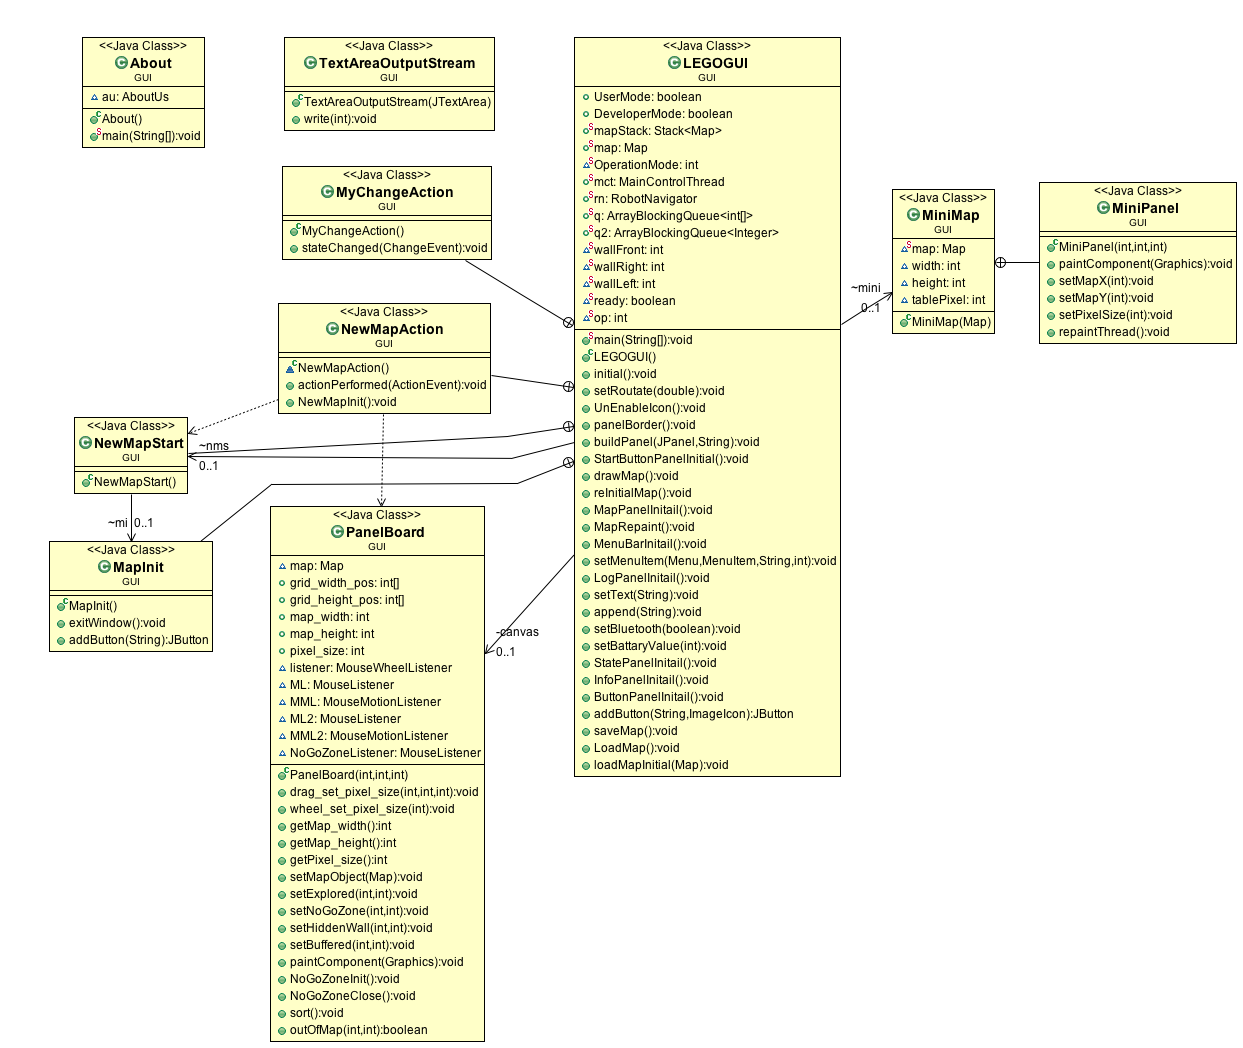
\includegraphics[width =0.8\linewidth]{GUI}}
\caption{Overview of the graphic user interface}
\label{sec:GUI}
\label{fig:GUI}
\end{figure}

The Graphic User Interface is a Java-Based Program, which is used to control robot from the host computer. The UI Window has a menu bar on the top, and a display panel under it.
The menu bar contains three menus: “File”, “Edit” and “Help”. Under the “File” menu contains options to open and save map, it can control the window as well. “Edit” menu has some functions to control the robot, User/developer mode switch and connection settings. “Help” menu contain an “about” item which shows the information of the software.
The main desk panel contains the map display area. Right side panel contains log information, auto/manual mode switch button, battery and Bluetooth connection state, and direction control buttons. Bottom panel contains current coordinate of robot in map and speed slider bar. 

\pagebreak

\section{Hardware Interfaces}


\begin{figure}[ht]
\centering
\setlength\fboxsep{2pt}
\setlength\fboxrule{0.2pt}
\fbox{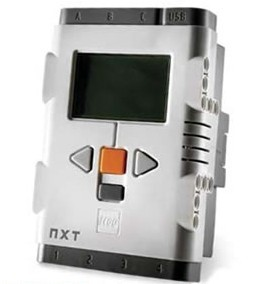
\includegraphics[width =0.6\linewidth]{brick}}
\caption{Hardware interfaces contains robot body (brick)}
\label{sec:BRK}
\label{fig:BRK}
\end{figure}

The brick has these four main interfaces:
\begin{itemize}
	\item{Bluetooth connection:}\\
	This part is the wireless communication device and data transfer device between user and robot. 
	\item{Light sensor:}\\
	Light sensor can detect the different stuffs on the map according their color depth.
	\item{Ultrasonic sensor:}\\
	Ultrasonic sensor is the device on the robot which looks like two “eyes”, it has the function like eyes as well. This device can sense the barrier in front of the robot, and it will warn the user if the bot is too close to the barrier. It can also let the bot stop through software when danger located in front of the bot.
	\item{USB interface:}\\
	USB interface has the same function as the Bluetooth. The difference is the data transfer and communications are both via a USB cable.
\end{itemize}
\pagebreak
\section{Software Interfaces}
Any machine (Mac/Windows/Linux) installed Java virtual machine(JVM) can run the software. GUI supports the LeJOS Java API and can be operated by the user, to implements this, the machine are required capable at either Bluetooth or USB connection. Real maps can be created, load and save map file through the GUI.


\section{Communications Interfaces}
Bluetooth (wireless) or USB (cable) connection can be connected to the robot. 
Files manipulation and other communication can be made through LeJOS NXJ Control Centre like this: 

\begin{figure}[ht]
\centering
\setlength\fboxsep{2pt}
\setlength\fboxrule{0.2pt}
\fbox{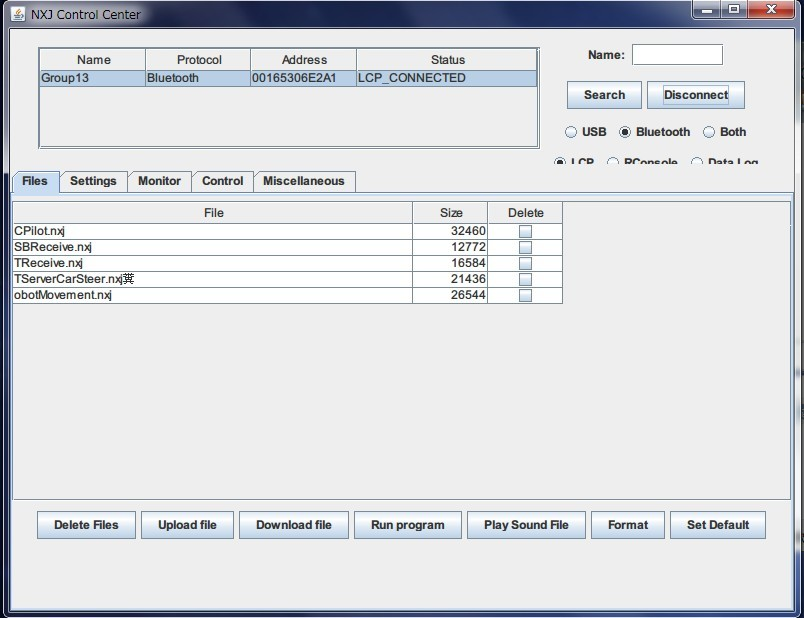
\includegraphics[width =0.8\linewidth]{NXJ_Control_Center}}
\caption{NXJ Control Center}
\label{sec:NXJCC}
\label{fig:NXJCC}
\end{figure}
With this program, basic connection can be made easily between host computer and brick. 
We can delete and upload testing source codes via either Bluetooth or USB cable.
\pagebreak


% Other Nonfunctional Requirements %

\chapter{Other Non-functional Requirements}


\section{Robot Performance}

\subsection{N0001: Time Performance}
\paragraph{Description:}
The robot must be able to scan the whole map and detect all the elements on that map, within a adequate amount of time.
\paragraph{Rational:}
Normally the robot should complete any tasks in 20 minutes, including scan the map and find all hidden walls and remnants.
\paragraph{Priority:}
Low

\subsection{N0002: Accuracy Performance}
\paragraph{Description:}
The robot must be able to mark the position of elements correctly and accurately. It must be able to tell the difference between hidden walls and remnants which distinguished by different colors.
\paragraph{Rational:}
The map must be generated correctly to allow the robot to avoid obstacles, even entering the no-go zones.
\paragraph{Priority:}
Medium

\section{Safety Requirements}

\subsection{N0003: latency}
\paragraph{Description:}
Robot is able to give a response to the command in a response time. Normally,this time is as short as possible.
\paragraph{Rational:}
Response time could be extremely important when the robot is in a dangerous situation and emergency stop needs to be carried out.
\paragraph{Priority:}
High

\subsection{N0004: Manual Mode Security}
\paragraph{Description:}
When the robot is in manual mode, the sensors must keep functioning to avoid collision or entering no-go zones. A warming message should also appears on GUI when the user is trying to do something dangerous.
\paragraph{Rational:}
Accident may happened in manual mode by misoperations. Even the user try to enter no-go zones or hit the walls intentionally, the robot should be able to stop by itself.
\paragraph{Priority:}
High 

\section{Safety Requirements}
\subsection{N0005: Mapping Safety}
The robot must not leave the map or enter the "no-go" zone. However, when the robot found itself in a "no-go" zone by accident or condition change of the site, it will send an error message to the host machine, stop the opreation and wait fot rescue.



\subsection{N0006: Action Safety}
The robot should not bump any blocks(walls etc.). Also the robot can not move against the user's will.  The robot is not allowed to be damaged at all the time.


\subsection{N0007: System Safety}
The system of the robot should have a encryption so that no one can hack it. Also the information robot gets will only send to the user, so no one can steal the information.


\subsection{N0008: System Update }
The system of the robot should be able to update or maintain in order to upgrade its security level. It can be updated by the user.


\subsection{N0009: Robot Design}
The robot should be designed sensibly and stably so that it will not be effected by the change of environment. Also a good design can help the robot move smoothly.


\subsection{N0010: Battery(Optinal)}
It is better if the robot has a power saving module. Also the robot should be fully charged before it is put to work. If the robot run out of power, it will go back to the initial point.



\section{Other Requirements}
\subsection{N0011: Speed}
The robot walks in normal speed, when the sensor detect the wall, robot will slow down. Moreover, the user can change the speed of the robot if he wants to.

\subsection{N0012: Sensors}
The default state of manual mode will be all sensors are set to on in order to countinue survey. However, if the user wishes to switch off the light sensor, they can do that. Under any circumstances, all the safety sensor such as ultrasonic sensor and touch sensor will stay on. 


\subsection{N0013: Accuracy}
The robot must map the archeological site accurately. It must has the ability to identify accurately
what it detect. (Above ground walls, buried walls, foundations)  With the accurate action, the robot can detect all the things in the site.


\subsection{N0014: Optimised Performance(Optional)}
It is better if the robot can Optimise the path after the survey(find the shortest way to reach the destination). This performance can save power and times.


\section{The GUI layout}

The GUI is desired to ensure that it is comfortable to used by our client. So we put directional control on the right-hand side same with keyboard as these buttons may be used most commonly. We also let the map occupies a lot of space to make sure users can see it clearly.

The GUI is fit into a 1100x768 fixed sized window with a 800x600 map display area. Speed control,icon information and Coordinate panels are located below the map.Log information, mode switching,NXT state and manual control buttons are on the right part.


\pagebreak

% Appendicies %
\newpage
\appendix

\pagebreak

\chapter{Glossary}

\textbf{Automatic Mode}:  Mode of operation, completely controlled by robot and host machine, without human input of movements. 
\\ \textbf{Bluetooth}: Wireless connection used to communicate between robot and host machine.
\\ \textbf{Explored Area}: The area that robot have inspected, which allows robot to travel safely.  
\\ \textbf{Gird}: A size of 50mm*50mm area in map, which contains 4 pixels. Each gird can be labeled as explored, unexplored, or "no go".
\\ \textbf{GUI}: Graphical User Interface. Displays the map panel, control panel and status panel.
\\ \textbf{Light Sensor}: Sensor used to detect hidden walls within the site, located at the front of the robot. The sensor returns the distance of the object.
\\ \textbf{Manual Mode}: Mode of operation. Movements controlled directly through operator.
\\ \textbf{"no go" zone}: A zone predefined is forbidden for the robot to enter. 
\\ \textbf{Pixel}: A size of 25mm*25mm area in map, defined as the smallest resolution, which is also the smallest area of hidden walls that robot can detect.  
\\ \textbf{SDD}: Software Design Document.
\\ \textbf{SEP}: Software Engineering and Project.
\\ \textbf{SPMP}: Software Project Management Plan.
\\ \textbf{Ultrasonic Sensor}: Sensor used to detect walls and obstacles within the site, located at the front of the robot. The sensor returns the distance of the object.
\\ \textbf{Unexplored Area}: The area that robot have not inspected, which can be considered dangerous.  
\\ \textbf{XML}: Extensible Markup Language. The map is saved as an XML file.





\end{document}

